\begin{problem}{Samliggjandi Tölur}{Inn}{Út}{~}{~}

	\begin{wrapfigure}{r}{0.35\textwidth}
		\vspace{-25pt}
		\begin{center}
			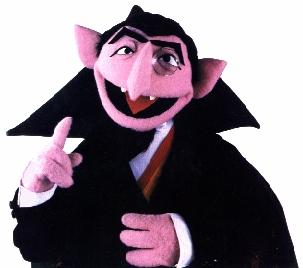
\includegraphics[scale=0.53]{../SamliggjandiTolur/count.jpg}
		\end{center}
		\vspace{-30pt}
	\end{wrapfigure}

	Jón litli er orðinn leiður á að gera heimalærdóminn sinn í stærðfræði. Hann tekur sér blað og blýant og byrjar að skrifa niður runu af samliggjandi tölum. Hann byrjar á tölunni 1 og heldur áfram alveg þar til hann kemur að tölunni $N$. Eftir það telur hann hversu oft hver tölustafur ($0$ til $9$) kemur fyrir í rununni. Tökum sem dæmi þegar $N = 13$. Þá skrifar hann niður rununa:
	\[12345678910111213\]
	Í þessari runu kemur $0$ einu sinni fyrir, $1$ kemur sex sinnum fyrir, $2$ kemur tvisvar sinnum fyrir, $3$ kemur þrisvar sinnum fyrir, og hver tölustafur frá $4$ til $9$ kemur nákvæmlega einu sinni fyrir. Eftir að hafa gert þetta í nokkurn tíma fer Jóni aftur að leiðast. Núna vill hann búa til forrit sem gerir þetta fyrir sig. En eins og hefur áður komið fram, þá kann Jón litli ekki að forrita! Hann biður þig því um að hjálpa sér.

	\Input

		Á fyrstu línu er heiltalan $1 \leq T \leq 20$, sem táknar fjölda prófunartilvika sem fylgja. Hvert prófunartilvik samanstendur af einni línu sem inniheldur heiltöluna $1 < N \leq 10000$.

	\Output

		Fyrir hverta prófunartilvik á að skrifa út eina línu. Línan inniheldur tíu tölur, aðskildar með bili. Fyrsta talan táknar hversu oft tölustafurinn $0$ kemur fyrir í rununni, annar tölustafurinn táknar hversu oft tölustafurinn $1$ kemur fyrir í rununni, og svo framvegis.

	\Examples

\begin{example}
\exmp{%
2 
3 
13
}{%
0 1 1 1 0 0 0 0 0 0
1 6 2 2 1 1 1 1 1 1
}%
\end{example}

\end{problem}